\section{Pitch and timbre}
\bi

\i \underline{Demonstrations}:
http://www.personal.psu.edu/meb26/INART50/psychoacoustics.html

\i \ques 
What distinguishes one musical tone from another?

\i \ans
duration, pitch, timbre, loudness or intensity, attack and 
decay transients, others (??)

\i We talked about loudness in a previous section.  
In this section we focus on pitch and timbre.

\i We shall see that the attack and decay transients 
affect the timbre of a tone.
Also one needs a duration of about 5 cycles to be able to 
determine the pitch of a tone.

\i Pitch is simply how high or how low (bass) a tone is.
It is a one-dimensional attribute (the frequency of the 
fundamental).

\i To describe timbre or tone quality, one uses words 
like ``bright" or "dark" $\cdots$, which are much more vague.
It is multi-dimensional attribute.

\ei

%%%%%%%%%%%%%%%%%%%%%%%%%%%%%%%%%
\subsection{Perfect pitch}
\bi

\i Perfect (or absolute) pitch:
Ability to determine the absolute pitch 
of a sound without regard to a reference tone.
Only about 1 out of 10,000 people in the population has perfect pitch. 

\i It is much more common for a person
to have {\em relative} pitch, which is the 
ability to determine the pitch of a sound
relative to some reference tone.

\i There is controversy regarding the origin
of perfect pitch.
Possible theories:
(i) it is hereditary,
(ii) it can be acquired through training, 
even in old age,
(iii) everyone has perfect pitch when they are
born, but it is lost through neglect, i.e., 
without training,
(iv) anyone can be taught to have absolute 
pitch if it is done at the right stage in 
their development (i.e., imprinting as a child).

\ei
%%%%%%%%%%%%%%%%%%%%%%%%%%%%%%%%%%%%%%%%%%%%%%%
\subsection{Pitch discrimination}
\bi

\i {\em Just noticeable difference} (JND) in frequency:
the minimum difference in the frequencies of 
two pure tones played sequentially that can
be distinguished from one another.

\i At high frequencies (i.e., above about 1000~Hz), the 
JND is approximately 0.5\% of the center frequency,
corresponding to roughly 1/10th of a semitone.
At low frequencies (i.e., below about 500~Hz), the 
JND is approximately 3~Hz, independent of the center frequency.
(See Figure~\ref{f:jnd_pitch}.)

\begin{figure}[htbp]
\begin{center}
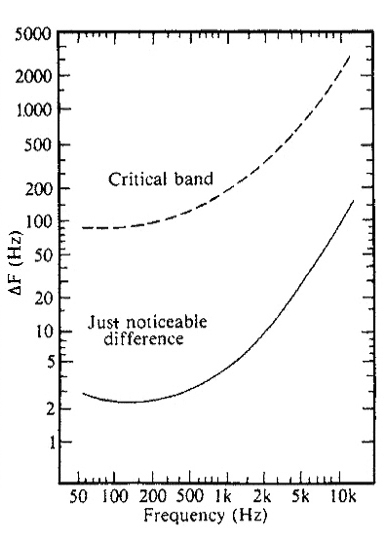
\includegraphics[width=.4\textwidth]{freqJNDa.jpg}
\caption{Just noticeable difference in frequency
and comparison to the critical bands on the cochlea.
(Figure taken from ``Science of Sound," by Rossing, Moore, and Wheeler.)}
\label{f:jnd_pitch}
\end{center}
\end{figure}
%

\i \ex From the figure, we see that at 2000~Hz 
the JND is approximately 10~Hz.
At 200~Hz the JND is approximately 3~Hz.

\i The JND has the same general dependence on 
frequency as does the critical bandwidth 
for the cochlea, but the JND is about a factor 
of 30 times smaller than the critical bandwidth.
(Recall: At high frequencies, 
the critical bandwidth is about 
15\% of the center frequency, corresponding
to one-fourth of an octave, or 3 semitones.
For example, at 2000~Hz, the critical bandwidth
is approximately 300~Hz.)

\i {\em Limit of frequency discrimination} (LFD):
the minimum difference between two pure tones 
played simultaneously that can be distinguished
from one antother.

\i The limit of frequency discrimination 
is about
$10\%$ of the center frequency, corresponding
to about 2 semitones.

\i Analogy: The sense of touch on the skin of 
your forearm using two pencil erasers separated 
by some distance.  

\i \demo 
Do the pencil eraser experiment.
Note that it is harder for you to tell if the pencil 
erasers are touching different parts of your forearm
if the erasers touch your skin at the same time.

\ei

%%%%%%%%%%%%%%%%%%%%%%%%%%%%%%%%%%%%%%%%%%%%%%%%%
\subsection{Missing fundamental and second-order beats}
\bi

\i If a complex tone containing many 
harmonics---{\em but not the fundamental}---is played, 
a person will identify the pitch of the sound to be 
that of the missing fundamental.

\i The missing fundamental is inferred by the
the brain from the timing of electrical impulses 
triggered by the periodicity of the complex 
sound wave.
(Recall that a complex sound wave containing
many harmonics---but not the fundamental---still 
has a period equal to the inverse of the 
fundamental frequency.
This is true even though the sound wave 
{\em does not have any power at the fundamental 
frequency.})

\i \demo Illustrate this with the matlab routine
{\tt fouriersynthesizeScript.m} for wave type
`missing'.

\i The missing fundamental does not correspond to
a physical wave in the ear.
The missing fundamental is an example of the 
{\em periodicity theory} of pitch. 

\i Contrast this to the {\em place theory} of 
pitch, which says that the pitch of a sound is
determined by the location on the basilar
membrane that is excited by the sound wave.
But if the sound wave doesn't contain power at
a particular frequency, then that part of the
basilar membrane won't be excited.

\i \exer
A complex tone consists of harmonics
200~Hz, 300~Hz, 400~Hz, etc.
What pitch will be heard?

\i \exer
A complex tone consists of the harmonics
300~Hz, 500~Hz, 700~Hz, etc..
What pitch will be heard?
(Hint: These are odd harmonics.)

\i \ans 100~Hz for both of the exercises.

\i Ordinary ({\em first-order}) beats are heard when
two pure tones with nearly identical frequencies
$f_1$ and $f_2$ are played simultaneously.
We hear beats at a frequency given by
%
\be
f_b = |f_1-f_2|
\ee
%
corresponding to alternating
periods of constructive and destructive interference.
We are sensitive to the low frequency
($<10~{\rm Hz}$)  amplitude modulation of a tone with 
frequency $\bar f = (f_1+f_2)/2$.

\i {\em Second-order} beats arise when two pure tones 
with frequencies that are nearly one octave apart, 
i.e., $f_2\approx 2f_1$, are played simultaneously.
We hear beats at a frequency given by 
%
\be
f_b=|2f_1- f_2|
\ee
%
The beats are a result of periodicity processing 
within the brain just like for the missing fundamental.

\i \demo 
Using the matlab routine {\tt playintervalFreq.m}, 
produce sounds with frequencies: 
(i) $f_1=440~{\rm Hz}$ and $f_2=442~{\rm Hz}$.
Listen for beats.
(ii) Repeat for $f_1=220~{\rm Hz}$ and $f_2=442~{\rm Hz}$.
For both cases, we hear beats with a frequency of 2~Hz.
The brain processes the periodicity of the combined waveform.

%\i \demo Illustrate the above cases graphically 
%using the matlab routine {\tt beats.m} using freuqencies
%(i) $f_1=10~{\rm Hz}$ and $f_2=11~{\rm Hz}$, and
%(ii) $f_1=5~{\rm Hz}$ and $f_2=11~{\rm Hz}$.

\ei
%%%%%%%%%%%%%%%%%%%%%%%%%%%%%%%%%%%%%%%%%%%%
\subsection{Aural harmonics and aural combination tones}
\bi

\i Asymmetries in the amplitude response of the 
human ear cause a pure tone to be represented
by a distorted wave having harmonics of the 
original sine wave.
These are called {\em aural harmonics}.

\i Aural harmonics are not part of the original
pure tone.
They are created by the non-linear 
amplitude response of the ear to sound pressure:
%
\be
x(t) = a_0 + a_1 p(t) + a_2 p^2(t) + a_3 p^3(t) + \cdots
\label{e:nonlinear}
\ee
%
where $a_n$ are constants.

\i Figure~\ref{f:auralharmonics-pure} 
shows a pure tone $p(t) = \sin(2\pi f t)$ 
with $f=1~{\rm Hz}$, and the non-linear 
output $x(t)$ for the special case $a_0=0$, $a_1=1$,
$a_2=1/2$, $a_3=1/3$, with all higher-order 
$a_n=0$.
Note that $x(t)$ is not a simple sinusoid.
%
\begin{figure}[htbp]
\begin{center}
\begin{tabular}{cc}
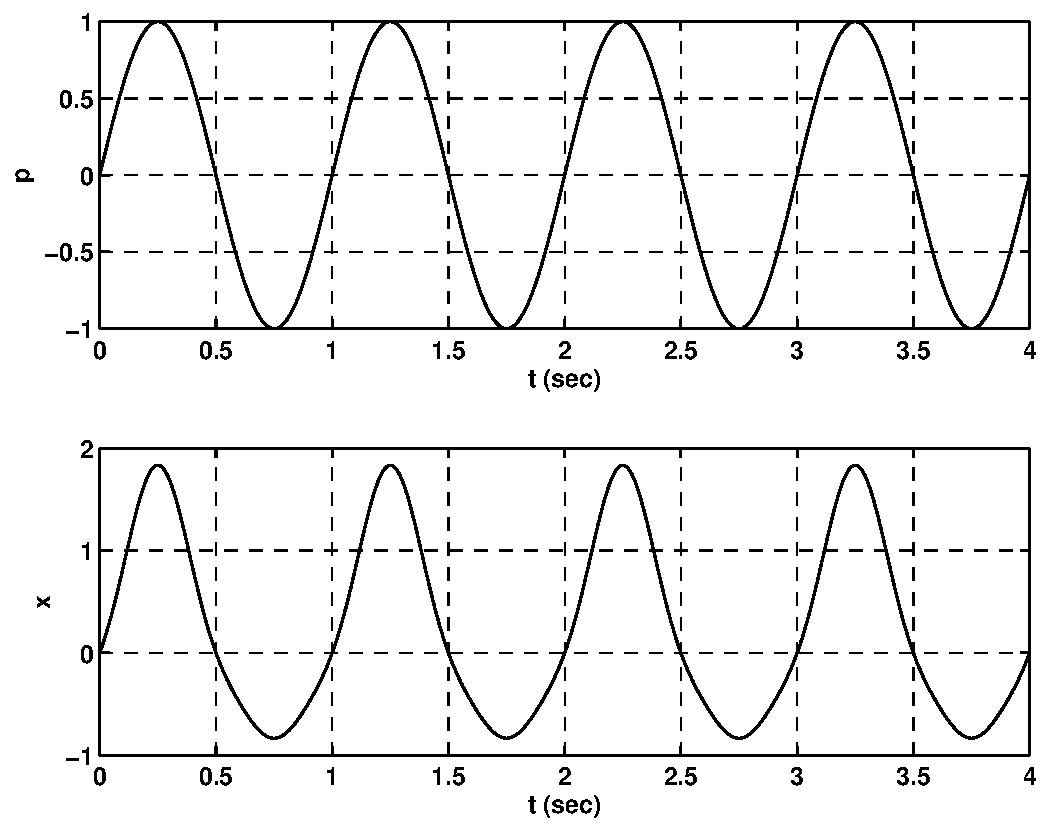
\includegraphics[width=.45\textwidth]{auralharmonicstime_pure} &
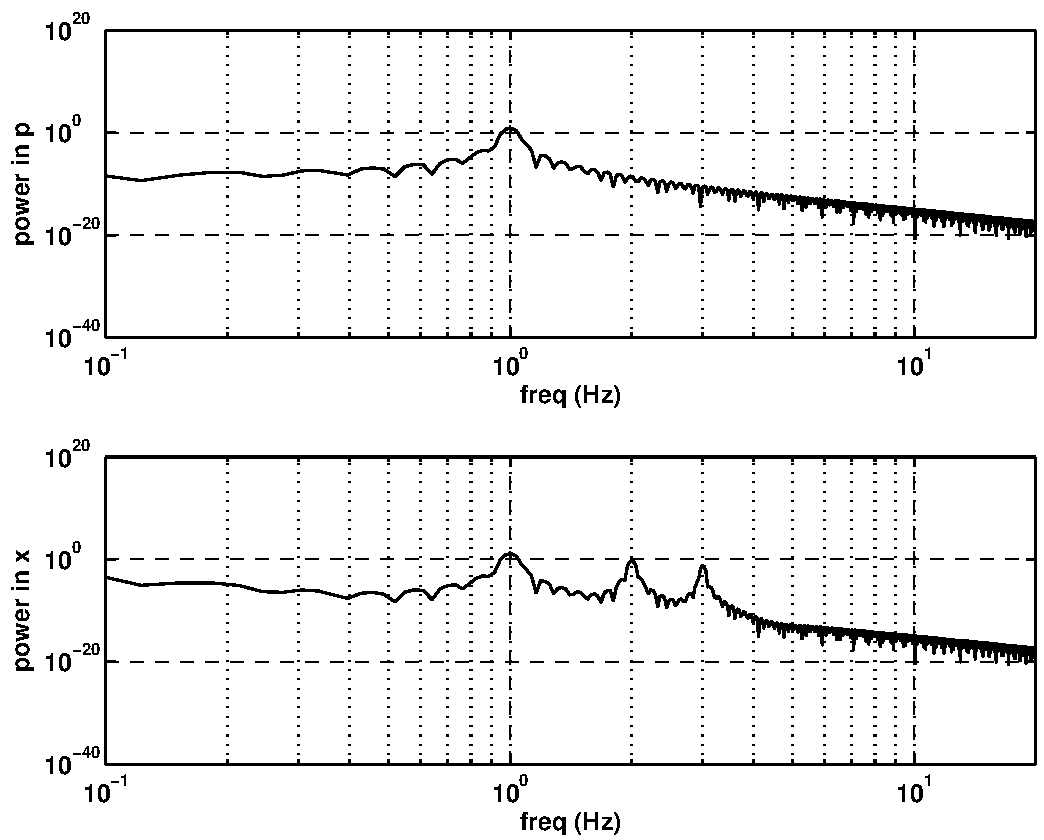
\includegraphics[width=.45\textwidth]{auralharmonicsfreq_pure}
\end{tabular}
\caption{Illustration of aural harmonics produced by
the non-linear response of the ear.
Top two panels: pure sinusoidal input and its corresponding
frequency spectrum.
Bottom panels: non-linear output and its corresponding 
frequency spectrum containing linear, quadratic, and cubic contributions.}
\label{f:auralharmonics-pure}
\end{center}
\end{figure}
%
\begin{figure}[htbp]
\begin{center}
\begin{tabular}{cc}
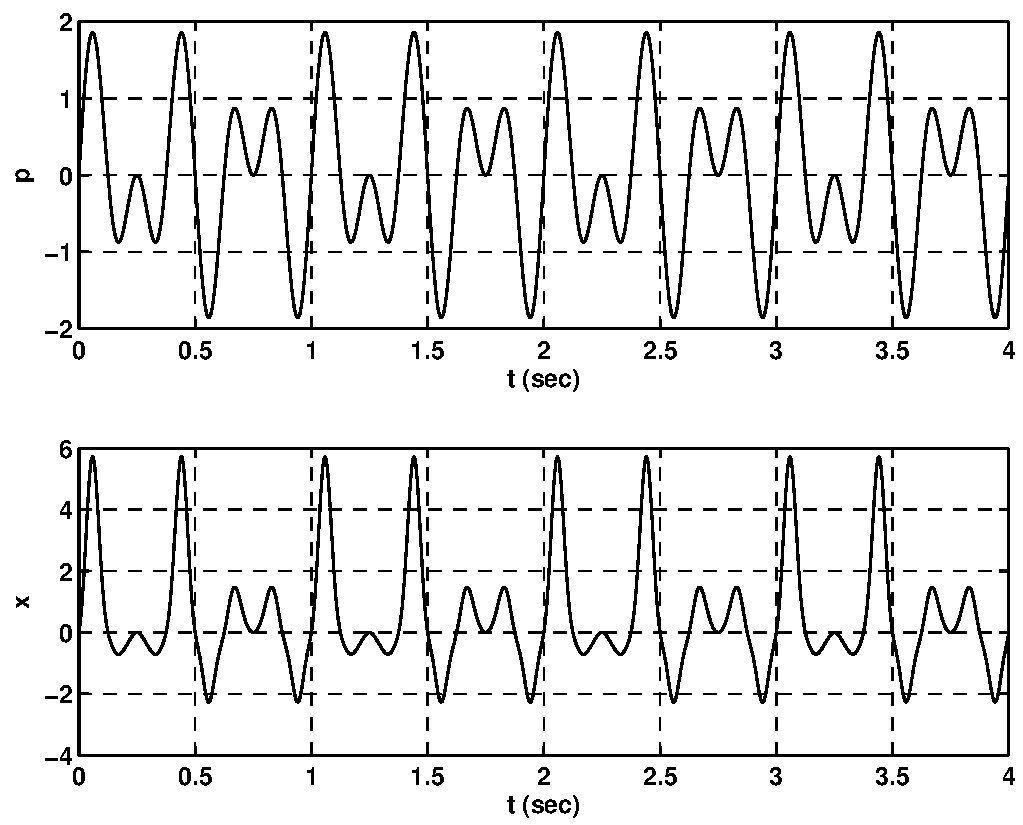
\includegraphics[width=.45\textwidth]{auralharmonicstime_complex} &
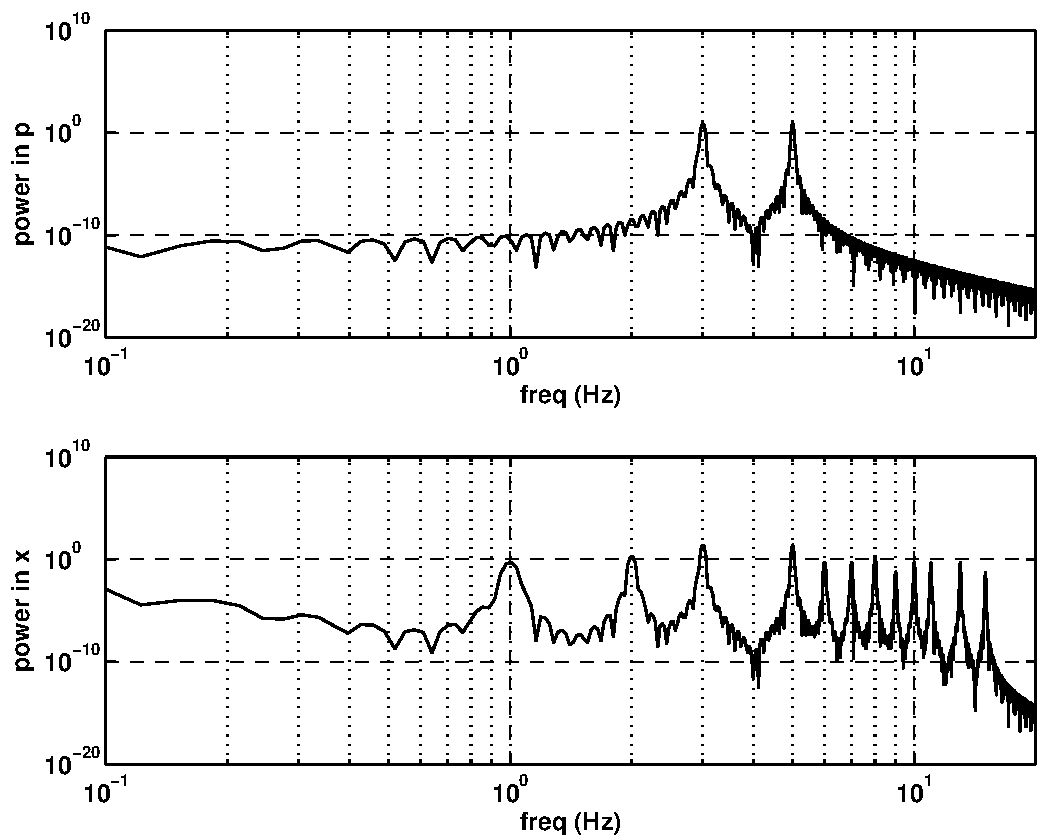
\includegraphics[width=.45\textwidth]{auralharmonicsfreq_complex}
\end{tabular}
\caption{Same as the previous figure, but for a complex
tone consisting of a sum of two sine waves with frequencies
$f_1=3~{\rm Hz}$ and $f_2=5~{\rm Hz}$.
From the bottom-right-hand plot we see that the 
non-linear output has contributions from several different 
combination 
tones $f_c= |mf_1 \pm nf_2|$, ranging from 1~Hz to 15~Hz.
There is no contribution from 4, 12, or 14~Hz for this 
particular example, where $x(t)$ contains only linear, quadratic,
and cubic terms.}
\label{f:auralharmonics-complex}
\end{center}
\end{figure}


\i If two pure tones (with frequencies $f_1$ and
$f_2$) are played sufficiently
loudly, then the non-linear response of the ear
will create aural {\em combination tones} having frequencies
equal to the sum and difference of the two original 
frequencies:
%
\be
f_c = |m f_1 \pm n f_2|
\ee
%
where $m$ and $n$ are integers.

\i Figure~\ref{f:auralharmonics-complex} illustrates 
this for a complex tone made up of two sinusoids with 
frequencies $f_1=3~{\rm Hz}$ and $f_2=5~{\rm Hz}$.

\i Combination tones exist as physical waves
having power at the sum and difference frequencies.
The difference tones are more easily heard 
than  the sum tones.
The effect is greatest when the two tones are loud.
The most easily heard difference tones have
frequencies given by
%
\be
|f_1-f_2|\,,\quad
|2f_1-f_2|\,,\quad
|3f_1-f_2|
\ee

\i \ex
Play two notes simultaneously on a piano 
a fifth apart, e.g., C${}_4$ and G${}_4$.
The frequencies differ by (approximately) a factor of 3/2.
If the two notes are played sufficiently loudly,
one hears the difference tone C${}_3$, which is an octave 
below C${}_4$.

\i The fact that one can hear bass notes from a 
small loudspeaker is due to a combination of 
(i) the aural difference tone of adjacent harmonics, and 
(ii) our perception of the missing fundamental.

\i \underline{Application}:
This is an advantage for speaker manufacturers, 
as well as for manufacturers of pipe organs,
since to physically produce the lowest bass
notes would require extremely long organ pipes.
We let the ear and the brain create the lowest
bass notes from the higher-order harmonics.

\ei
%%%%%%%%%%%%%%%%%%%%%%%%%%%%%%%%%%
\subsection{Timbre}

\bi
\i Timbre (or tone quality) can be defined as 
``Any attribute that allows a listener to
judge that two sounds are disimilar using any criteria
other than pitch, loudness, or duration" (Pratt and Doak, 1976).

\i Timbre depends on the relative contribution
of the harmonics or overtones that make up the sound wave.

\i Aural harmonics introduced by non-linearities
in the ear change the timbre of a pure tone.

\i Ohm and Helmholtz did some experiments (in the 1800's)
showing that the timbre of a complex tone 
depends primarily on the amplitude of the harmonic
components and {\em not} on their relative phases.
This is called {\em Ohm's law of hearing}.

\i \demo Illustrate this using the matlab routine
{\tt fouriersynthesizesoundScript.m} with inputs
{\tt `sawtooth'} and {\tt `sawtoothphase'}.
 
\i Ohm's law of hearing is important for sound reproduction 
systems.
Although the process of sound recording and playback 
(which uses electromagnetic induction)
may change the relative phases of the harmonics, 
the played-back sound sounds virtually identical to that 
of the original sound.

\i Timbre also depends on the {\em attack} and 
{\em decay transients} of the sound.

%\i \demo Illustrate this by playing sounds with the attack 
%transients removed
%(track 2 of the soundtrack from John Powell's book, ``How music works").
%Can you guess what instrument that is?

\i A note from an instrument sounds different if it is played 
forward or backward in time.

\i \demo Illustrate this using the matlab routine
{\tt playrecordedsound(`pianoC4',0)} and\\
{\tt playrecordedsound(`pianoC4',1)}.

\i \demo Also play\\
{\tt playrecordedsound(`happybirthday', 0)} followed by\\
{\tt playrecordedsound(`happybirthday-backwards',0)}, and\\
{\tt playrecordedsound(`happybirthday-backwards',1)}.

\ei
%%%%%%%%%%%%%%%%%%%%%%%%%%%%%%%%%%%%%%%
\subsection{Consonant and dissonant tones}
\bi

\i Two complex tones are consonant (sound pleasing) when several
of the harmonics or overtones coincide.

\i Consonance / dissonance depends on the frequency difference
bewteen the two tones and not on the frequency ratio.
If the frequency difference is greater than the critical
bandwidth, then the notes sound consonant.
If the frequency difference is slightly less than the critical
bandwidth, then the notes sound rough.
If the frequency difference is roughly equal to a quarter
of the critical bandwidth then the notes have maximum
dissonance.

\i \ex C to G is a fifth, which always has a 
frequency ratio of (approximately) 3/2.

C$_4$ to G$_4$ has $\Delta f=130~{\rm Hz}$ which is
greater than the critical bandwidth 
$\Delta f_{\rm cb}\approx 100~{\rm Hz}$
at the center frequency $\bar f=328~{\rm Hz}$, 
and so sounds consonant.

C$_3$ to G$_3$ has $\Delta f=65~{\rm Hz}$ which is
slightly less than the critical bandwidth 
$\Delta f_{\rm cb} \approx 90~{\rm Hz}$
at the center frequency $\bar f=164~{\rm Hz}$,
and so sounds rough.

C$_2$ to G$_2$ has $\Delta f=32~{\rm Hz}$ which is
about one-third of the critical bandwidth 
$\Delta f_{\rm cb}\approx 90~{\rm Hz}$ 
at the center frequency $\bar f=82~{\rm Hz}$, 
and so sounds dissonant.

\i \demo Illustrate this using a dual function
generator, first for the frequencies 
$f_1 = 262~{\rm Hz}$ (for C${}_4$) and $f_2 = 392~{\rm Hz}$ (for G${}_4$);
then for
$f_1 = 131~{\rm Hz}$ (for C${}_3$) and $f_2 = 196~{\rm Hz}$ (for G${}_3$);
and finally for
$f_1 = 65~{\rm Hz}$ (for C${}_2$) and $f_2 = 98~{\rm Hz}$ (for G${}_2$).

\ei

%%%%%%%%%%%%%%%%%%%%%%%%%%%%%%%%%%%%%%%%%%%%%%
\subsection{A pitch paradox}

\bi

\i In 1964, Roger Shepard constructed a repeating set of complex
tones (called {\em Shepard tones}), whose pitch appears to increase 
(or decrease) forever.

\i \demo Illustrate this with the matlab routine
{\tt shepardscale(`ascending',1)}.

\i \demo Also watch the YouTube videos by David Huron 
(http://vimeo.com/34749558).

\i The Shepard scale is the musical analog of the optical 
illusion of a
{\em never-ending staircase}, 
originally developed by the mathematician
Lionel Penrose in 1958, and subsequently used by M.C.~Escher in
his 1960 print `Ascending and Descending.'
(See Figure~\ref{f:penrose-staircase} of a never-ending staircase.)
%
\begin{figure}[htbp]
\begin{center}
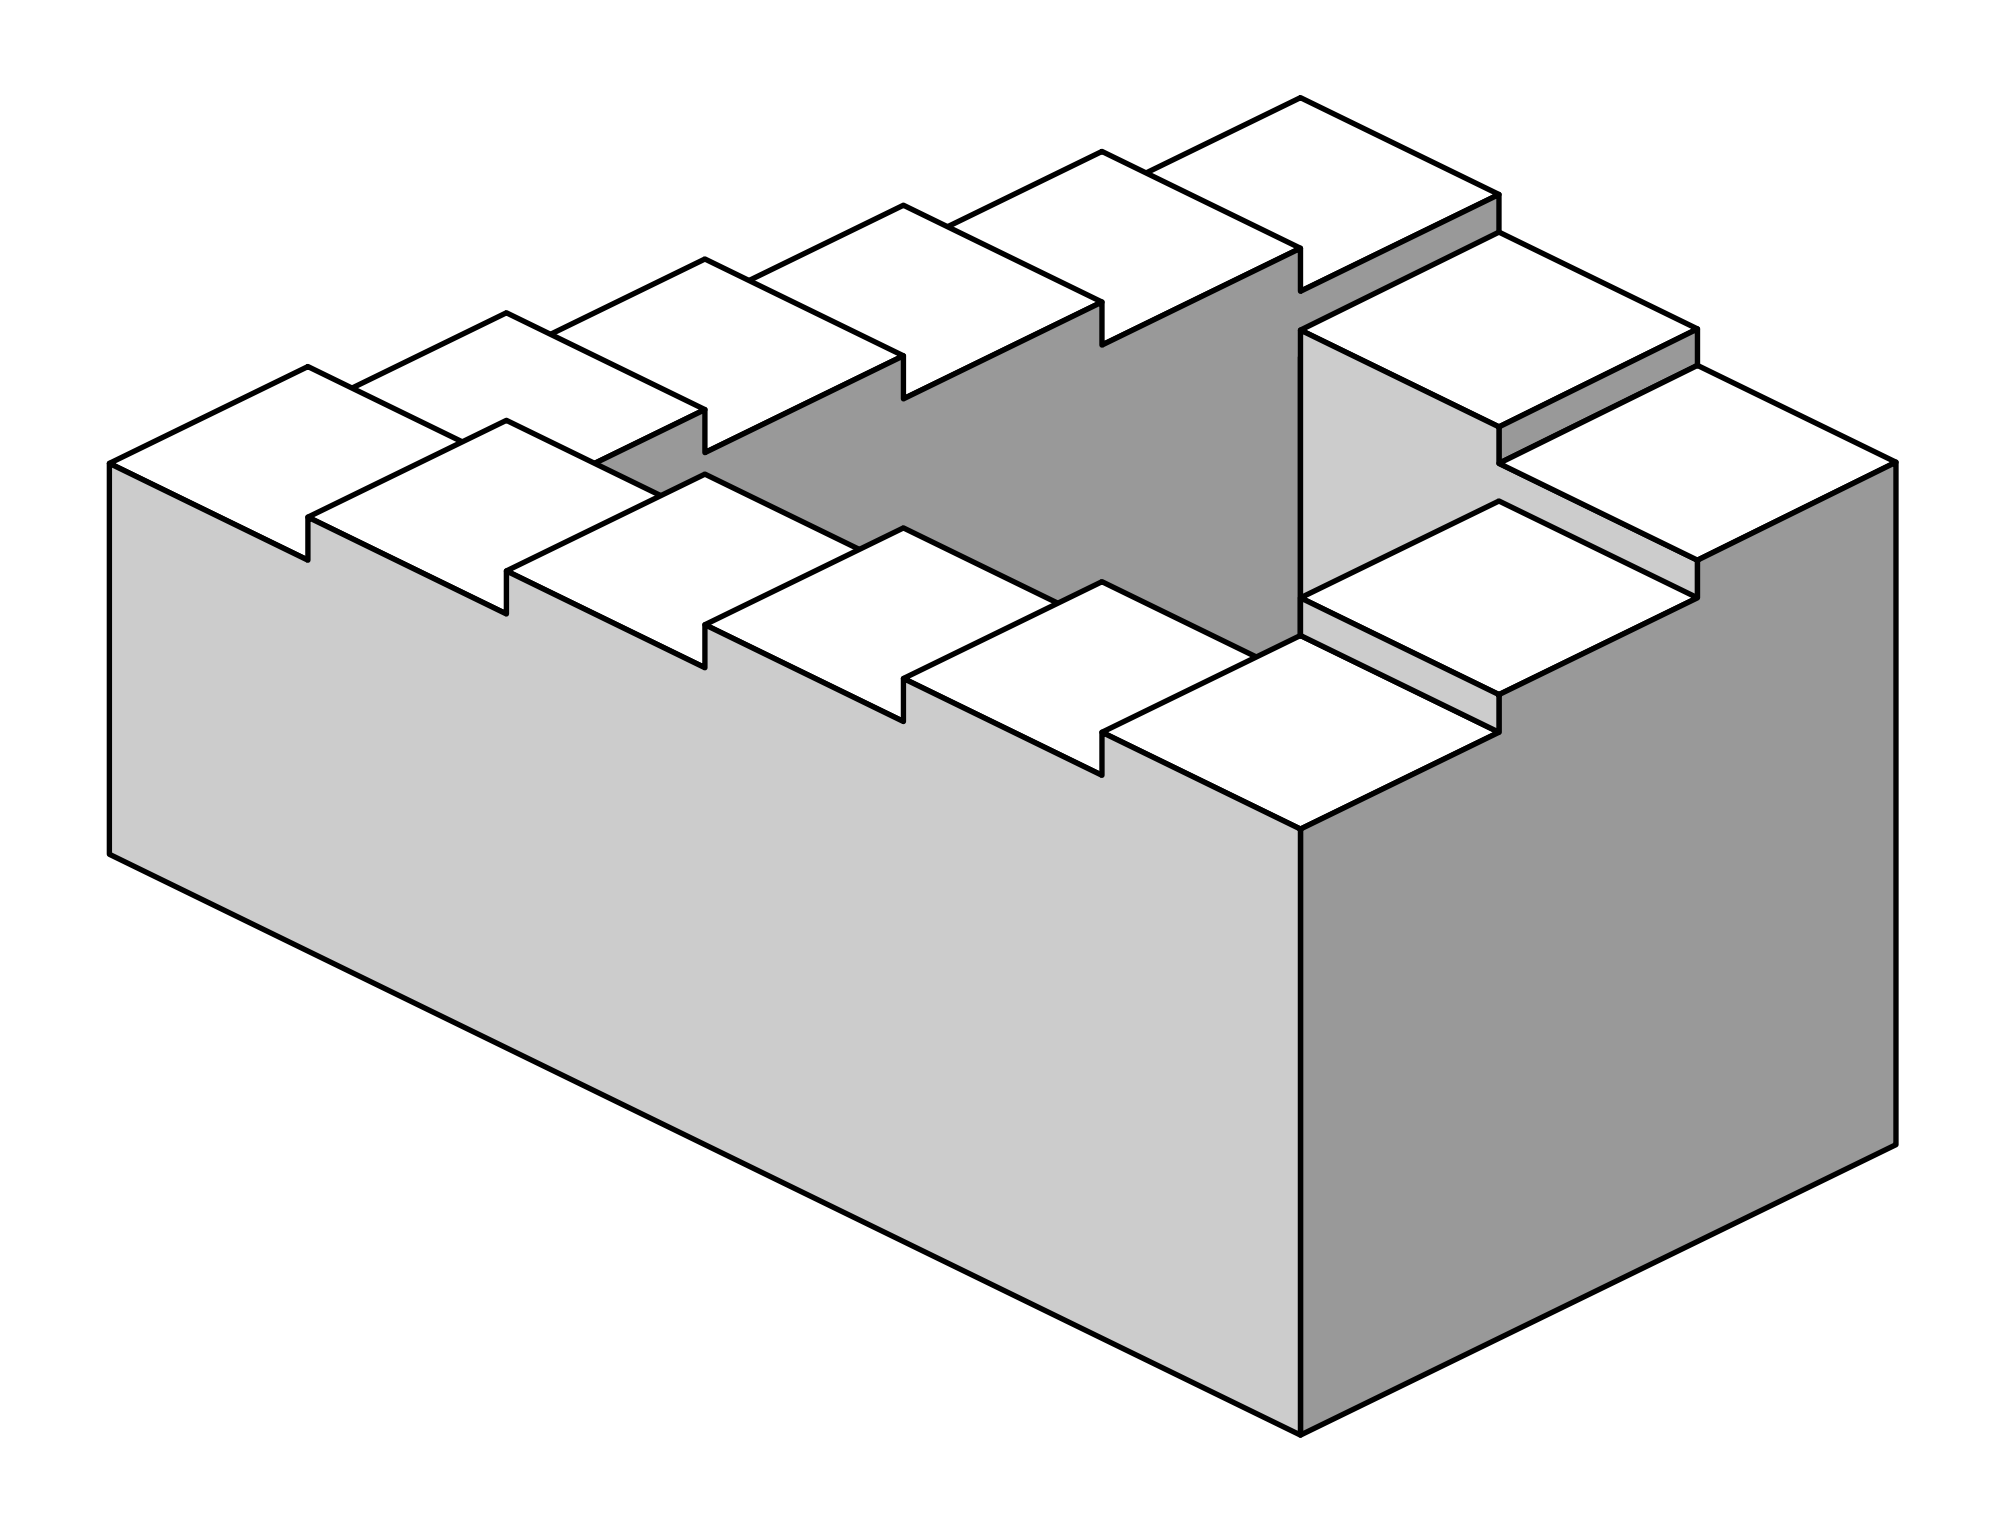
\includegraphics[width=.4\textwidth]{penrose-staircase.png}
\caption{Never-ending staircase.}
\label{f:penrose-staircase}
\end{center}
\end{figure}
%

\i \demo Watch the YouTube vide called the Shepard-Penrose mix\\
(http://www.youtube.com/watch?v=PCs1lckF5vI)

\i \ques How does the Shepard scale work? 

\i \ans EXTRA CREDIT, 2 points for an explanation.

\ei
